
\subsection{実験の目的,概要}
本実験では,16ビット加算回路を順序回路で記述し,機能レベルシュミレーションと論理合成を実行する。
これによって,出力値が仕様を満たしているかどうか,論理合成による回路構成を確認する。

入力は,clk(1bitクロック),reset(1bitリセット信号),x,y(16bitオペランド),y(1bit桁上げ入力)。
出力は,sum(16bit演算結果),cout(1bit桁上げ出力)。
ただし,入力値の演算結果は次のクロックの立ち上がりで出力に反映させる。

ICE計算機上の,ModelSim,Quartusを使用する。

順序回路の設計法と回路合成結果の確認を行い,実験2の結果と比較することで,等価な回路が設計によって,どのように異なるかを考察することを目的とする。

\subsection{実験方法}
\subsubsection{回路のHDL記述}
以下のような回路記述をadder16s.v,テストベンチをtest\_adder16s.vとして作成した。
\lstinputlisting[caption=adder16s.v,label=adder16s.v]{./src/adder16s/adder16s.v}
\lstinputlisting[caption=test\_adder16s.v,label=testadder16s.v]{./src/adder16s/test_adder16s.v}

\subsubsection{機能レベルシュミレーション}
作成したテストベンチをもとに,ModelSimで信号波形を出力した。
入出力の値が仕様通りの真理値表と一致することを確認した。

\subsubsection{論理合成}
以下の2ファイルを作成し,配置した。
\lstinputlisting[caption=adder16s.qpf,label=adder16s.qpf]{./src/adder16s/adder16s.qpf}
\lstinputlisting[caption=adder16s.qsf,label=adder16s.qsf]{./src/adder16s/adder16s.qsf}

作成した回路記述をQuartusでコンパイルし,論理合成とレイアウトを行った。
回路構成やロジックエレメント数,遅延時間について確認した。
 
\subsection{実験結果}
\subsubsection{機能レベルシュミレーション}
ModelSimで波形を作成した結果,以下のような波形になった。

\begin{figure}[H]
  \centering
  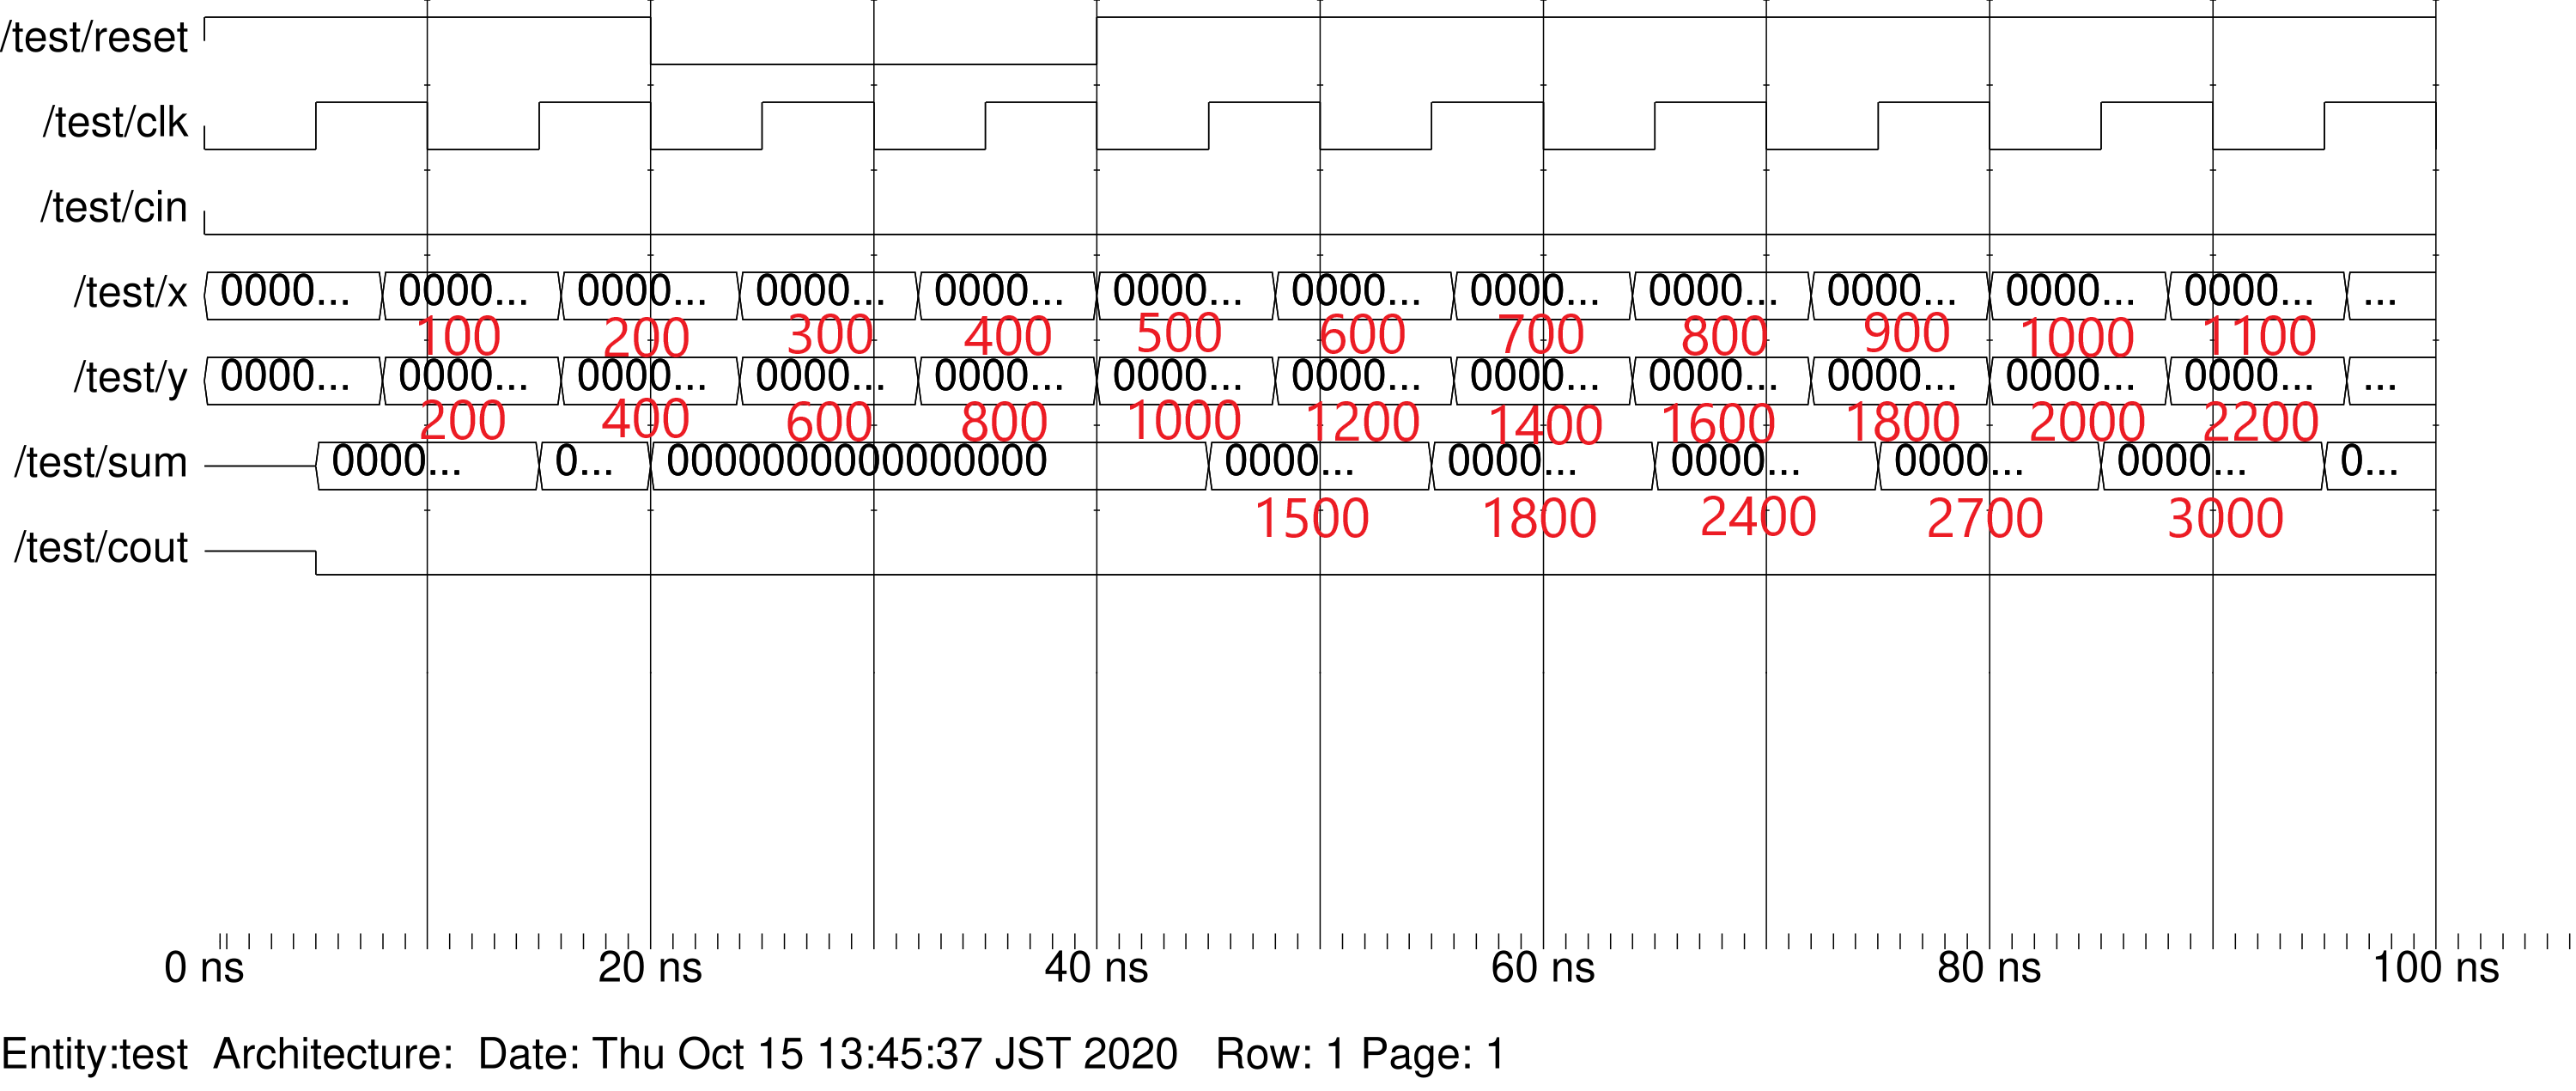
\includegraphics[width=\linewidth]{./src/adder16s/adder16s_wave31.png}
  \caption{adder16sの波形}
\end{figure}

\subsubsection{論理合成}
論理合成の結果,以下のような回路が作られた。

\begin{figure}[H]
  \centering
  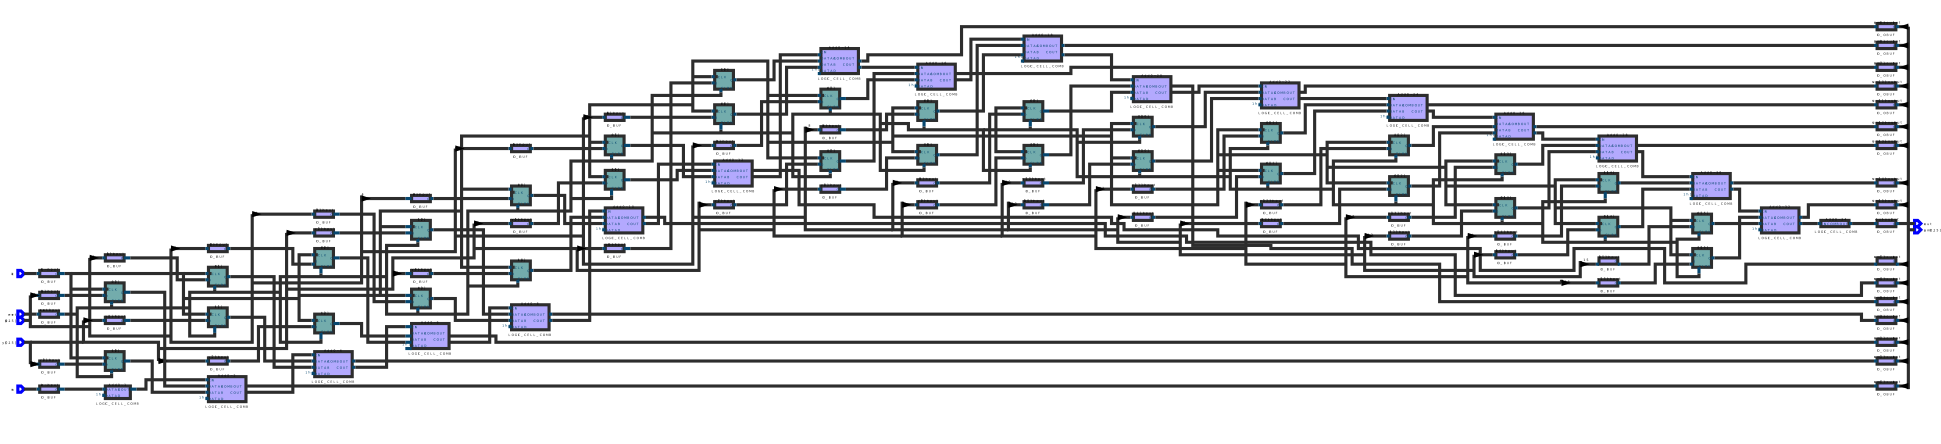
\includegraphics[width=\linewidth]{./src/adder16s/adder16s_print.png}
  \caption{adder16sの回路}
\end{figure}

ロジックエレメント数は35だった。

回路全体の遅延時間は,以下のようになった。

\begin{figure}[H]
  \centering
  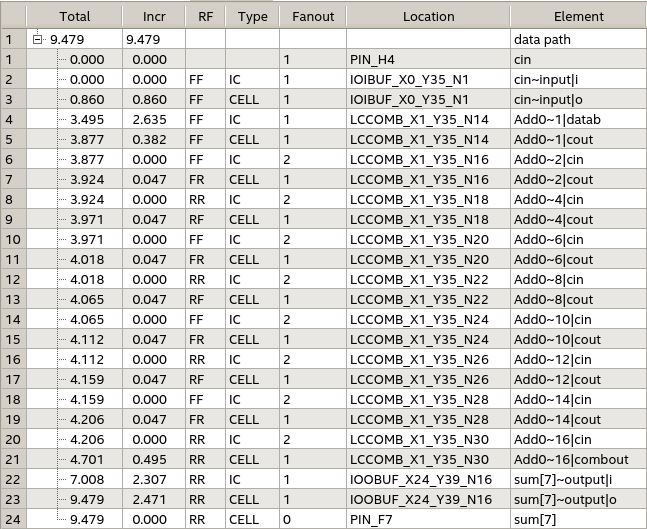
\includegraphics[width=\linewidth]{./src/adder16s/adder16sTiming.png}
  \caption{adder16sの遅延時間}
  \label{adder16sの遅延時間}
\end{figure}

\subsection{考察}
\subsubsection{回路のHDL記述}
コード\ref{adder16s.v}では,クロックの立ち上がりで,定義した2つの16bitレジスタに入力x,yの値を代入している。
その結果がコード\ref{adder16.v}と同様にassignされているので,クロックに同期して動作すること以外は,\ref{adder16.v}と同じである。

また,リセット信号の立ち下がりでレジスタの値はリセットされる。

コード\ref{testadder16s.v}ではテストベンチとして,5nsごとにクロック信号を反転している。
(10nsごとに回路が動作する)

また,8nsごとにxに100を加算し,yに200加算している。

\subsubsection{機能レベルシュミレーション}
クロック信号に対応して出力されていた。
また,リセット信号も正しく動作している。

\subsubsection{論理合成(実験2との比較)}
合成結果では,全加算器列と桁数*2個のフリップフロップによって回路が作られていた。
これによって,組み合わせ回路のときよりもロジックエレメント数は増加している。

一方で,全体の遅延時間は10\%程度減少している。
回路内で,全加算器の数は両方16個で,加算器のみの遅延は図\ref{adder16sの遅延時間}より0.047で,図\ref{adder16の遅延時間}の遅延時間と同じである。

しかし,順序回路では入力の変化に関係なく,クロックによってフリップフロップに保存される予定の,その瞬間の入力値が読み取られる。
つまり,クロックが入力されるまで,入力の値はフリップフロップのすぐ前に待機していると言える。
その結果として,実験3では最長パスが1桁目の全加算器から始まっている。
このような原因で,順序回路のほうが遅延は小さいと考えられる\\
